\documentclass[11pt]{article}

\usepackage[utf8]{inputenc}
\usepackage[T1, T2A]{fontenc}
\usepackage[english, serbianc]{babel}

\usepackage{biblatex}
\addbibresource{MLofi.bib}

\usepackage{graphicx}
\usepackage{longtable}
\usepackage{wrapfig}
\usepackage{rotating}
\usepackage[normalem]{ulem}
\usepackage{amsmath}
\usepackage{amssymb}
\usepackage{capt-of}
\usepackage{hyperref}
\author{Петар Никић, Вукан Антић}
\date{\today}
\title{Генерисање музике применом неуронских мрежа}
\begin{document}

\maketitle
\begin{abstract}
У овом раду демонстрирамо како се неуронске мреже могу користити за генерисање музике. Фокус рада је на генерисању мелодија за клавир. Приказане су две архитектуре: једна заснована на рекурентним неуронским мрежама и друга заснована на конволутивним неуронским мрежама. Крајњи модели су у стању да са делимичним успехом генеришу интересантне мелодије.
\end{abstract}

\section{Увод}
\label{sec:org3572ae7}
Прављење музике је задатак који је пре пар деценија био незамислив за рачунаре, и резервисан за човека због креативности коју човек поседује. Међутим, у скорије време, показано је да и машине могу да буду добри композитори (\cite{van_der_oord_wavenet_2016}).

Напредак на овом пољу омогућила је појава неуронских мрежа, и то посебних неуронских мрежа које раде са секвенцама података: рекурентним и конволутивним неуронским мрежама.

\section{Проблем}
\label{sec:org2995f58}
У овом раду бавимо се генерисањем музике из \emph{Lo-fi} жанра. Lo-fi (low fidelity) жанр одабрали смо због своје једноставности. Музика овог жанра се састоји из следећих елемената:
\begin{itemize}
\item Музичког узорка (sample)
\item Бубњева
\item Позадинских звукова
\end{itemize}

Музички узорак представља (обично кратки) низ тонова и акорда који се понављају током песме.

Узорак песми даје мелодију, бубњеви ритам, а позадински звукови се додају као стилски елемент жанра.

Фокус нашег рада је био генерисање управо музичког узорка употребом неуронских мрежа.

\subsection{Формулација проблема}
\label{sec:org5232f06}
Када размишљамо о музици, једна од карактеристика коју лако можемо уочити је да постоји одређена временска структура музике. Тонови нису независни, већ се заједно комбинују у дуже структуре.

Проблем постављамо на начин који је карактеристичан за проблеме који се баве секвенцама података (\cite{graves_generating_2013}, \cite{van_der_oord_wavenet_2016}). Модел учи функцију \(f\) која представља условну расподелу вероватноће за наредни тон ако су познати претходни тонови у секвенци.

Прецизније, нека је \(T\) дужина секвенце коју посматрамо, \(x_t\) представља улаз модела у тренутку \(t\), и \(x = (x_1, x_2, \ldots, x_T)\) представља секвенцу улазних вектора. Модел учи условну расподелу
$$
P \left \{ x_{T + 1} \mid x_1, x_2, \ldots, x_T \right\}
$$

\section{Имплементација}
\label{sec:org0afbf05}
Имплементација модела је рађена у програмском језику \emph{Python}, у \emph{Jupyter} свескама, на сервису \emph{Google Colaboratory}. Од библиотека смо користили \emph{Music21} за обраду музичких података и \emph{Keras} за дефинисање модела и рад са моделом.

Коришћен скуп података за учење је \href{https://www.kaggle.com/zakarii/lofi-hip-hop-midi}{Lo-Fi Hip Hop MIDIs}, који је саставио Zachary Katsnelson.

\subsection{Обрада улазних података}
\label{sec:orgf3cd130}
Подаци су организовани као колекција песама и узорака у MIDI формату.

\texttt{music21} библиотеку смо користили да из узорака издвојимо низове тонова, акорда и пауза из изворних MIDI фајлова.

Након тога, музичке елементе из свих узорака смо спојили у један низ, и пресликали (бијективно) у целе бројеве.

Из великог низа музичких елемената свих узорака смо издвојили секвенце дужине која одговара хиперпараметру \texttt{sequence\_length}, заједно са наредним елементом који се користи за проверу тачности ноте која је предвиђена на крају. Овде треба напоменути да ће неке секвенце садржати елементе из различитих песама, али смо проценили да је прихватљиво допустити ове случајеве, јер се ради о једном жанру музике, и претпоставка је да су узорци довољно слични.

У случају рекурентне архитектуре, цели бројеви улазних секвенци се кодирају у асиметричне бинарне атрибуте (\emph{one-hot} кодирање), док у конволутивној архитектури цели бројеви првобитно пролазе кроз \texttt{Embedding} слој, који сваку вредност пресликава у вектор, који се прослеђује даљим слојевима.

Наредни елемент се у оба случаја кодира one-hot кодирањем.

\subsection{Модел}
\label{sec:org94184e3}
Истражили смо две архитектуре модела, једну рекурентну и једну конволутивну. Рекурентна архитектура је заснована на архитектури описаној у раду \cite{graves_generating_2013}, док је конволутивна инспирисана \emph{WaveNet} архитектуром, коју је представио \emph{DeepMind} у \cite{van_der_oord_wavenet_2016}.

Модели су дефинисани функционалним апликативним програмским интерфејсом који нуди библиотека \emph{Keras}.

\subsubsection{Рекурентна архитектура}
\label{sec:orge6c52e7}
Рекурентна аритектура је организована у 4 скривена, рекурентна слоја. За рекурентне елементе се могу користити прости рекурентни елемент (RNN), Long Short-Term Memory (LSTM) или Gated Recurrent Unit (GRU).

У мрежу су додати скокови: улаз се прослеђује свим сем последњег скривеног слоја, и сви скривени слојеви прослеђују улаз последњем. На овај начин се смањује број корака од почетка до краја мреже, чиме се умањује проблем \emph{нестајања градијента}, и обезбеђује боље учење дубоких мрежа.

На крају се налази обичан, густи слој са \emph{softmax} активационом функцијом, који описује расподелу вероватноћа за наредни елемент секвенце (музички елемент).

\begin{figure}[htbp]
\centering
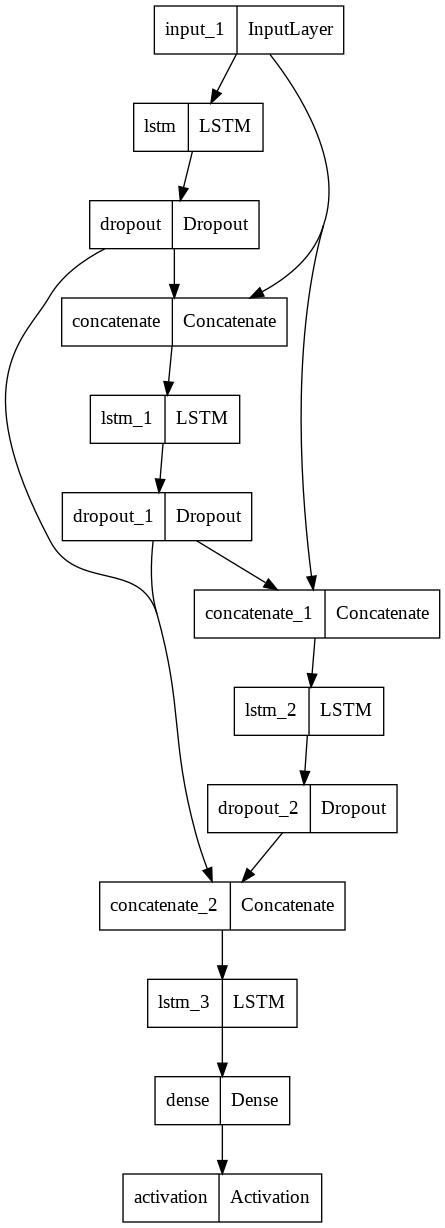
\includegraphics[scale=0.4]{./img/model-lstm.png}
\caption{\label{fig:org61e3d3d}Изглед рекурентне архитектуре}
\end{figure}

\subsubsection{Конволутивна архитектура}
\label{sec:org5c021fb}
Конволутивну архитектуру карактерише наизменични низ једнодимензионих конволуција са \(ReLU\) активационом функцијом и једнодимензионих \(\max\) агрегација.

Конволуције у моделу су узрочне конволуције са дилатацијом (causal dilated convolutions).

Узрочне конволуције резултат формирају искључиво на основу претходних вредности секвенце, што одговара полазном проблему у којем су зависности од прошлих ка будућим вредностима.

Дилатација омогућава да се на дубљим слојевима повећа ширина поља вредности на основу којих се врши предикција, односно број улазних вредности које учествују у предикцији. Шире поље нам је битно за учење дугорочне структуре података, које је природно присутно у рекурентним мрежама, али није у конволутивним. Други начини на који се може обезбедити шире поље су коришћење више слојева или увећавање филтера. Оба наведена случаја значајно повећавају количину потребног рачуна.

\begin{figure}[htbp]
\centering
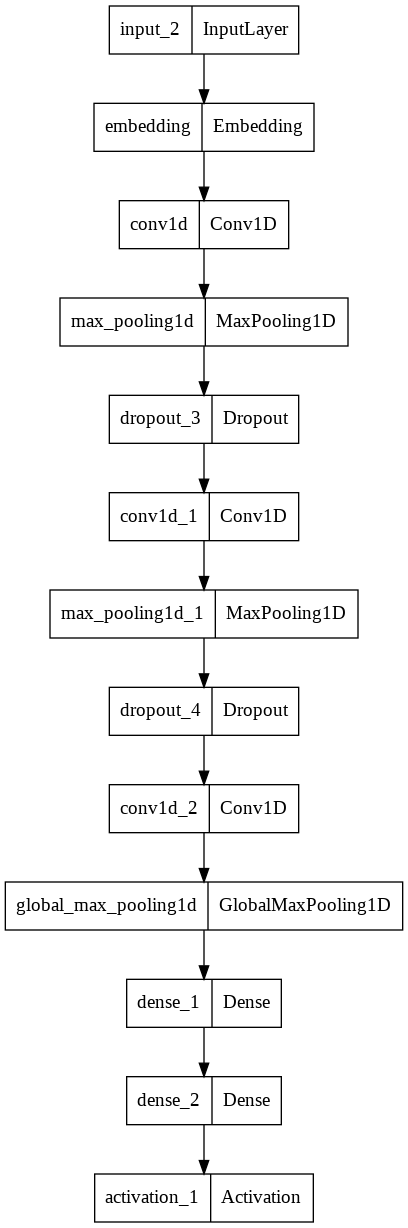
\includegraphics[scale=0.4]{./img/model-cnn.png}
\caption{\label{fig:orge30df59}Изглед конволутивне архитектуре}
\end{figure}

\subsection{Генерисање музике}
\label{sec:org9f53bbc}
Музика се генерише давањем иницијалног узорка који представља замишљене ноте пре почетка генерисања.

На основу узорка се генерише следећа нота, узорковањем из расподеле коју дефинише излаз мреже. Узорак се помера ка прошлости, прва нота се избацује, а на место последње ноте се смешта генерисана нота, након чега се нови узорак може користи за даље генерисање наредних нота.

\section{Резултати}
\label{sec:orgfd96aa2}
У току развоја цео скуп је коришћен за тренирање. Скупови за валидацију и тестирање нису коришћени. Први разлог за доношење такве одлуке је мањак података. Додатном поделом скупа података би се додатно смањио доступан број података за тренирање. Други разлог је због природе проблема који решавамо. Музика је субјективна ствар, и сматрали смо да постоји шанса да модел који нема велику тачност прави бољу мелодију од модела који има велику тачност. Начин обраде података није потпуно природан, и доста поједностављује изворне податке, што даје додатне назнаке за претходно наведену тврдњу.

Прихватајући субјективне карактеристике музике, процену смо вршили генерисањем и слушањем узорака. Неки од резултата које смо приметили следе.

\begin{itemize}
\item Прости RNN елементи нису могли да адекватно моделују структуру музике, и генерисани узорци су често били једна или две ноте које се врте у петљи.
\item LSTM и GRU су показали сличне резултате, што је било и очекивано (\cite{chung_empirical_2014}). Субјективно, више су нам се допали резултати генерисани GRU моделом.
\item Конволутивни модел боље моделује локалну структуру музике, због чега обично звучи природније од рекурентних модела.
\item LSTM, GRU и CNN модели генеришу различите резултате за различите улазе. То је добар индикатор да могу да науче одређени стил, али да се не фиксирају за једну песму.
\end{itemize}

Међутим, главни утисак је да генерисана музика није на нивоу способности човека. Неопходна је обрада генерисаних резултата, попут одабира интересантних делова и исецање тих делова од остатка песме. Алтернативна употреба модела може да буде као инспирација за професионалне уметнике, који могу да очувају идеју иза генерисане музике, уз преправке грешака које начини модел.

\printbibliography

\end{document}
